\documentclass[jarticle]			% for platex
\usepackage[dvipdfmx]{graphicx}
% \documentclass[uplatex,dvipdfmx]{jlreq}		% for uplatex
\title{鉛直渦動粘性係数、拡散係数の比の変化による水温の変化の考察}
\author{工学部社会基盤学科 B4 石田紘大}
\date{\today}
\begin{document}
\maketitle

\section{各地点ごとでの水温コンターマップ}
シミュレーションにおいて、VPRNU(VERTICAL PRANDITL NUMBER)を変化させ、鉛直混合の変化を比較した。以下のコンターマップ(2ページ目)を作成した。\\
なお、測点はすべて千葉一号塔である。
\begin{figure}[hbtp]
    \begin{tabular}{cc}
    \begin{minipage}[t]{0.45\hsize}
     % \centering
        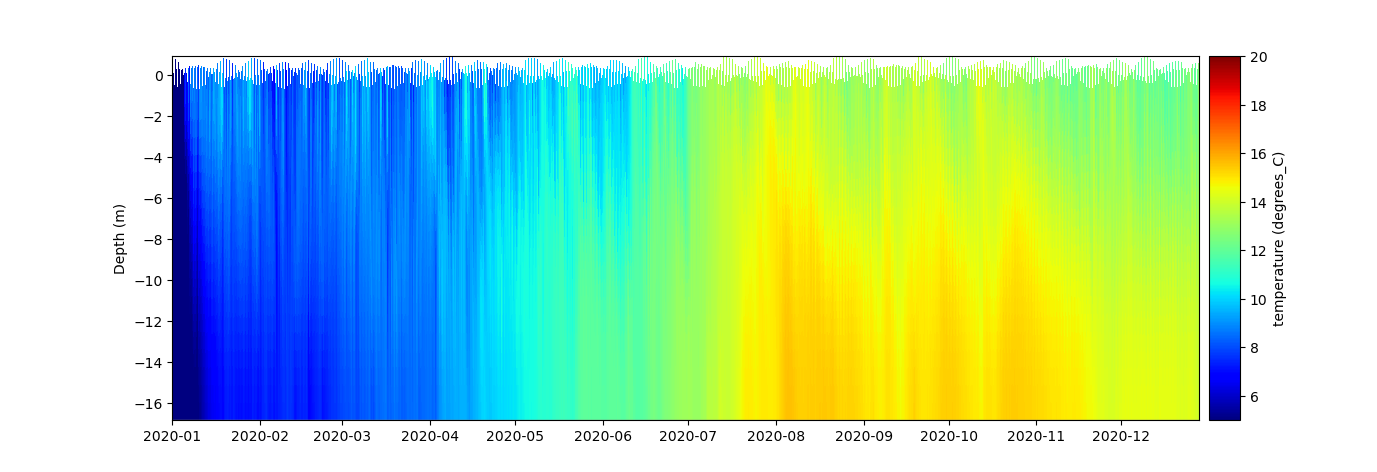
\includegraphics[width=160mm]
        {contour/Tokyo03_chiba1buoy.png}
       \caption{VPRNU=0.1,type=closure}
       \label{コンター03}
    \end{minipage} \\
    \begin{minipage}[t]{0.45\hsize}
      \centering
        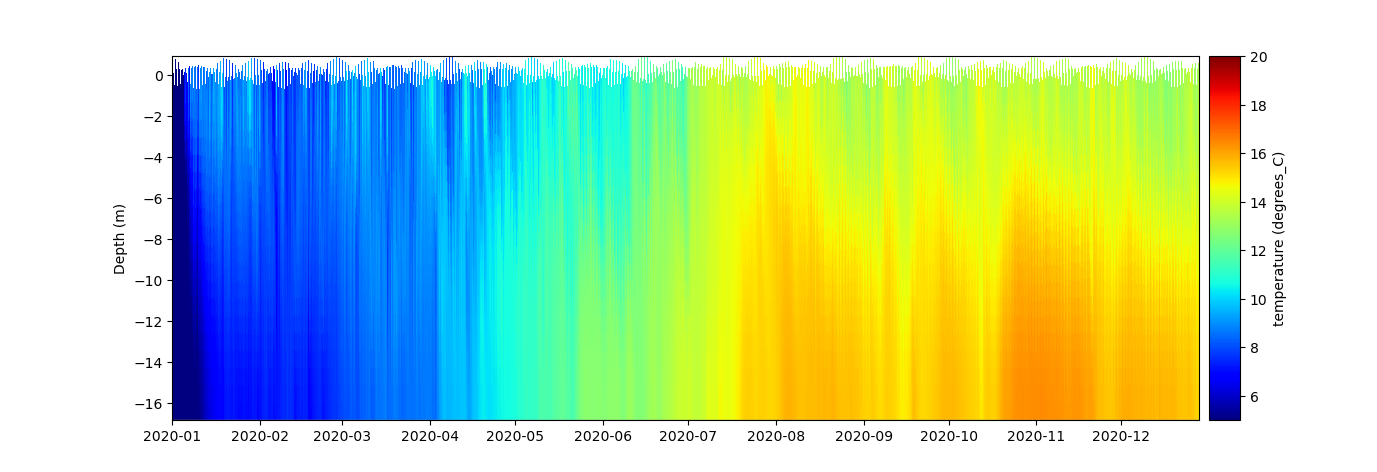
\includegraphics[width=160mm]
        {contour/Tokyo04_chiba1buoy.png}
      \caption{VPRNU=0.2,type=closure}
      \label{コンター04}
    \end{minipage} \\
    \begin{minipage}[t]{0.45\hsize}
      \centering
        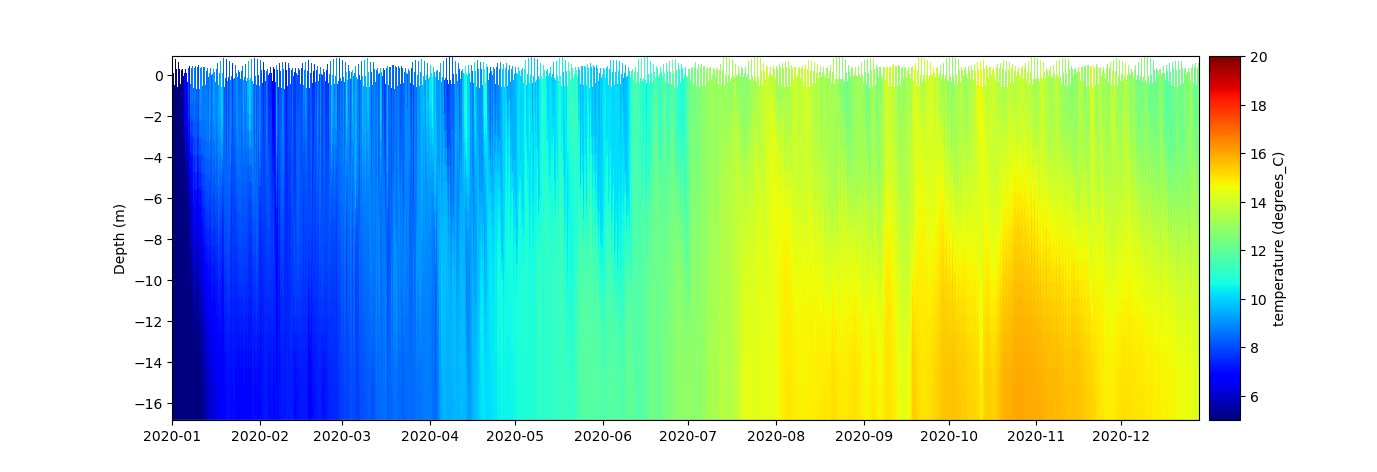
\includegraphics[width=160mm]
        {contour/Tokyo05_chiba1buoy.png}
       \caption{VPRNU=0.8,type=closure}
       \label{コンター05}
    \end{minipage} &
    
  \end{tabular}
\end{figure}


\section{VERTICAL\_mixing\_coefficient=1e-6}
一方、VPRNU=0.1,VERTICAL\_mixing\_coefficient=1e-6とした場合の結果は{1e-6}のようになった。

